%
% einleitung.tex -- Beispiel-File für die Einleitung
%
% (c) 2020 Prof Dr Andreas Müller, Hochschule Rapperswil
%
% !TEX root = ../../buch.tex
% !TEX encoding = UTF-8
%
Das Weltall hat uns Menschen und Mathematiker schon immer fasziniert und inspiriert. 
Seit Mitte des 20. Jahrhunderts ist es endlich möglich, Raketen in den Weltraum zu schicken. 
Dabei stellt die Berechnung der Flugbahn ein klassisches Variationsproblem dar. 
Ziel ist es, möglichst wenig Treibstoff zu verbrauchen, um den Wirkungsgrad zu maximieren.

In der Regelungstechnik gibt es viele solcher Variationsprobleme, doch die Komplexität einer Raketenflugbahn ist besonders herausfordernd. 
Sie hängt von zahlreichen Faktoren ab, wie dem Raketentyp und der Atmosphäre. 
Dieses Kapitel zeigt, wie man ein so komplexes Problem vereinfachen kann, um eine realitätsnahe Lösung zu erhalten. 
Es werden die Grundlagen der Bewegungsgleichungen und Randbedingungen untersuchen und die Techniken der Variationsrechnung anwenden, um die optimale Flugbahn zu finden. 
In Zukunft werden diese Berechnung wohl überflüssig dank dem Unendlichen Unwahrscheinlichkeitsantrieb.

\begin{figure}
	\centering
	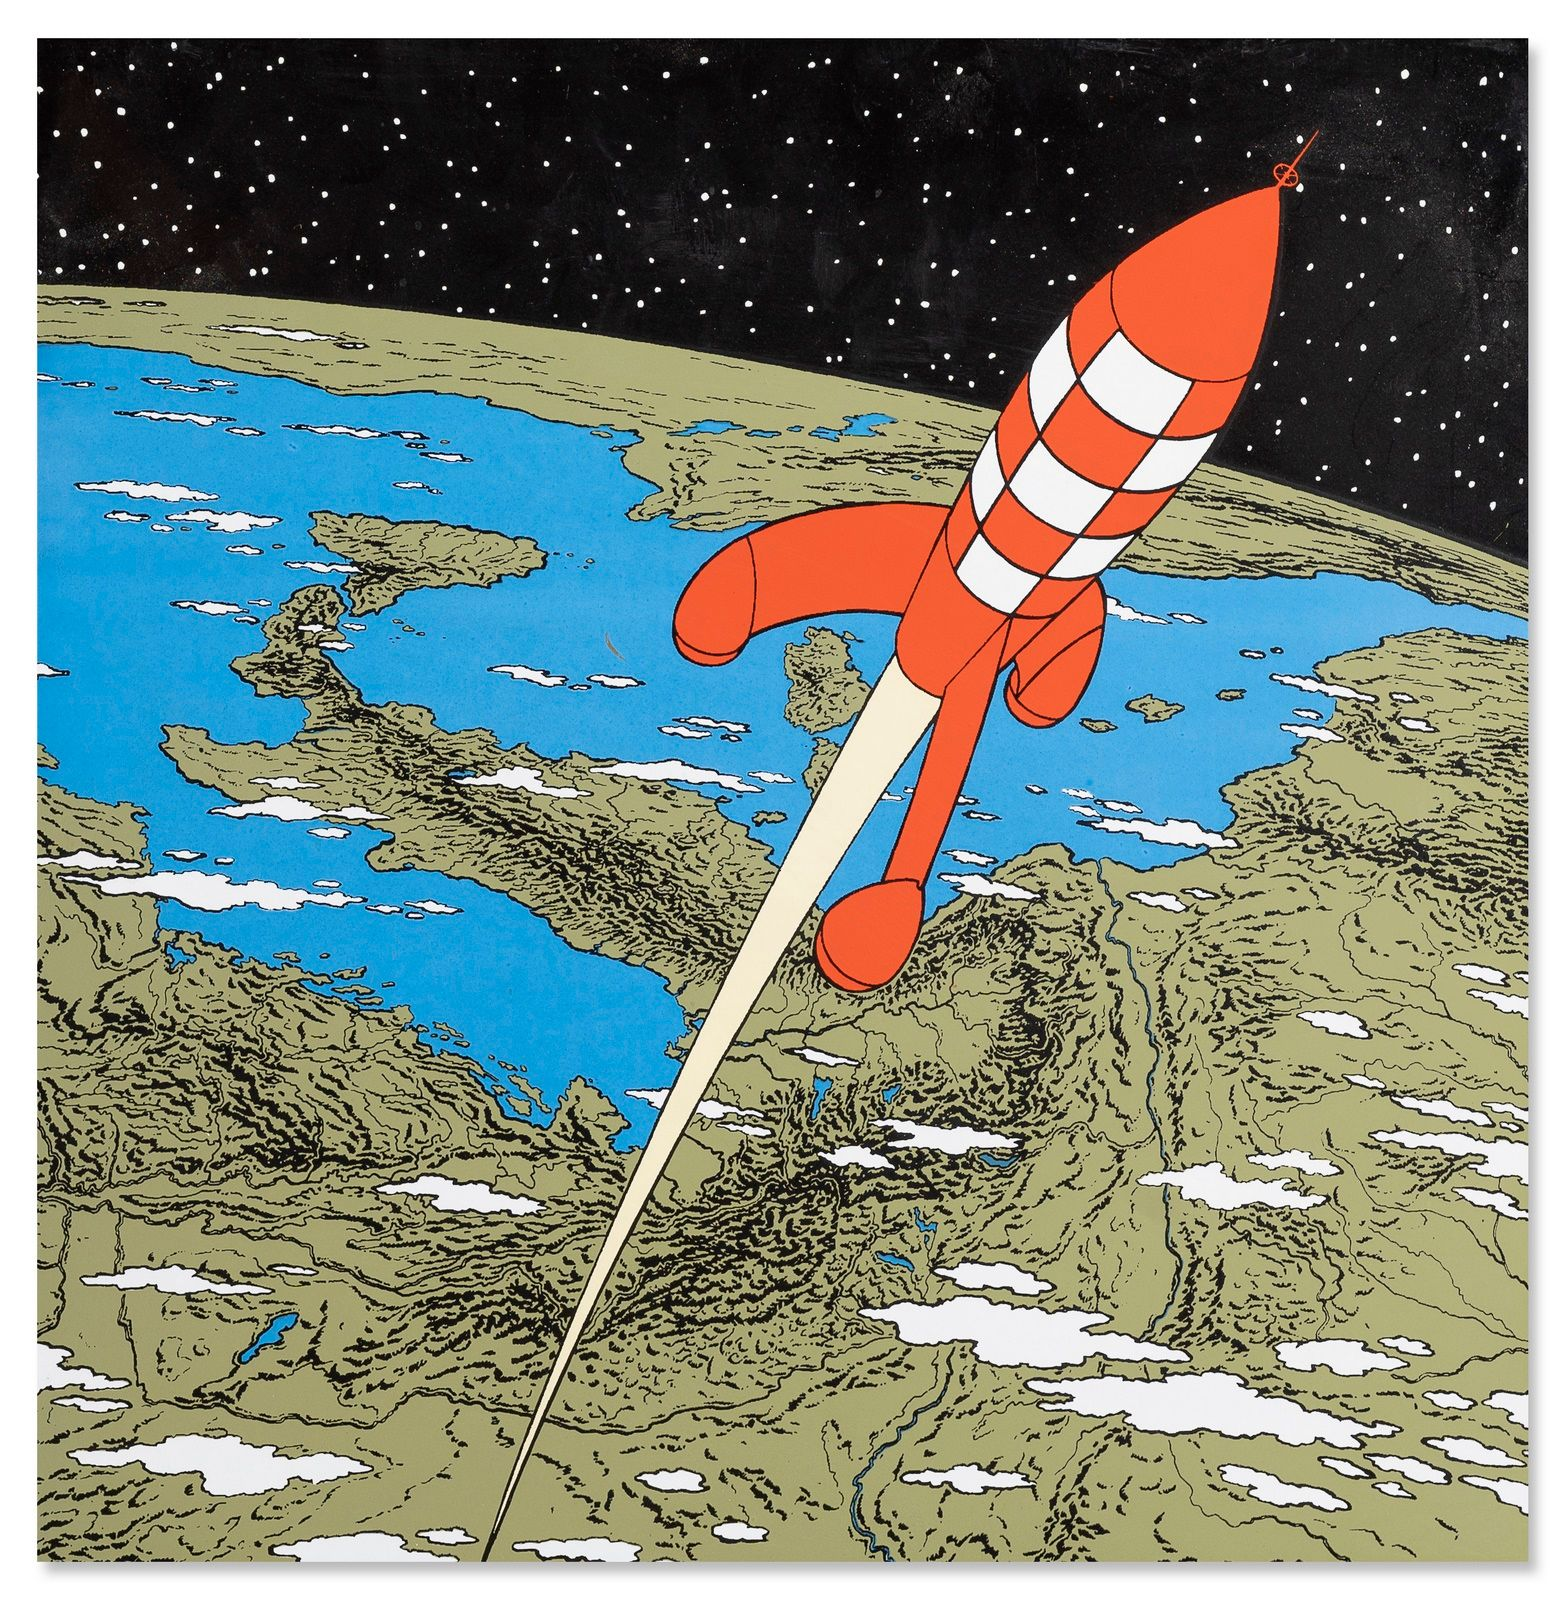
\includegraphics[width=0.4\linewidth]{papers/leo/Grafiken/raketen_typen.jpg}
	\caption{Als 1953 der Tim und Struppi Reiseziehl zum Mond erschien, war dies für viele Menschen noch unvorstellbar \cite{leo:timstruppi}.}
	\label{fig:leo:raketen_typen}
\end{figure}







